\documentclass{article}
\usepackage{amsrefs}
\usepackage{amssymb}
\usepackage{amsmath}
\usepackage{amsthm}
\usepackage{graphicx}

\newtheorem*{voorbeeld}{Voorbeeld} \newtheorem*{eigenschap}{Eigenschap} \newtheorem*{opmerking}{Opmerking}

\title{Oppervlakten berekenen met bepaalde integralen}
\date { }

\begin{document}

\maketitle \noindent

\noindent Stel dat de grafiek van een functie $f(x)$ er uit ziet als op de volgende figuur

Tekening uit de Actimath cursus blz 23 in 3.1.1

\noindent Uit de definitie van $\int ^b_a f(x)dx$ weten we dat 

Onderste twee regels uit de Actimathcursus blz 23 (dus de twee formules onder die tekening) gevolgd door de rest van de Actimath cursus uit 3.1.1 blz 24 en 25.\\

\noindent Algemener, als $f(x)$ en $g(x)$ twee functies zijn allebei continu op een interval $I$.
Stel dat $a$ en $b$ tot $I$ behoren met $a<b$.
Op de volgende figuur is de gearceerde oppervlakte de oppervlakte begrensd door de grafieken van $f(x)$ en $g(x)$ en de vertikale rechten $x=a$ en $x=b$.

\begin{figure}[h]
\begin{center}
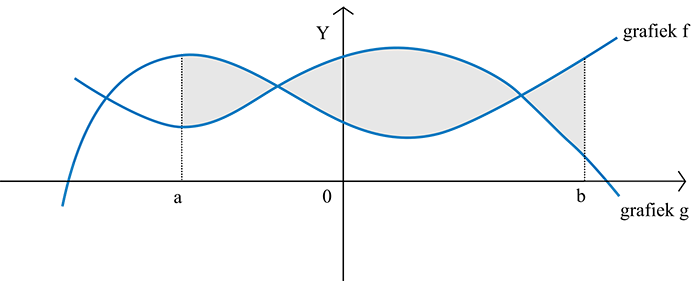
\includegraphics[height=5 cm]{integraal3.JPG}
\end{center}
\end{figure}

Deze oppervlakte bereken je met de volgende bepaalde integraal

$\boxed { \int^b_a \vert g(x)-f(x) \vert dx }$

Daarna uit de cursus Actimath de methode van blz 26.

\begin{voorbeeld}
Voorbeeld 1 uit de cursus Actimath op blz 26 en 27.
\end{voorbeeld}





\end{document}